%<><><><><><><><><><><><><><><><><><><><><><><><><><><><><><><><><><><><><><><><><><><><><>
 % Analysis of existing data
 %<><><><><><><><><><><><><><><><><><><><><><><><><><><><><><><><><><><><><><><><><><><><><>

\section{Analysis of existing data}
We investigated the challenges of reconstructing 2$\pi^0$ final states
with a missing recoil proton using the 2017 GlueX data taken with a
hydrogen target and the 2019 PrimEx-Eta data with beryllium and helium targets.
This is a useful exercise to verify that nearly elastic 2$\pi^0$
events can be detected with GlueX and to check the resulting
resolutions with real data. Unfortunately, the high backgrounds with these targets prevented the extraction of a Primakoff signal.
\subsection{Hydrogen target}
  We selected and reconstructed events that matched the
topology of the reaction $\gamma p\rightarrow \gamma \gamma \gamma
\gamma\, (p)$ with a missing proton. A kinematic fit was performed
that conserved energy and momentum and imposed a vertex constraint at the center of the target cell
($z=65$~cm). The fit was required to converge. We note
that even though the vertex was
fixed at 65~cm to perform the fit, the actual target extends from 50
to 80 cm. Several other nominal selection criteria were imposed to clean up
the event sample, including the absence of charged tracks and a requirement
that there be no missing
energy. No constraints were imposed on the $\pi^0$ mass to allow study of
backgrounds. In addition accidental background subtractions were performed.
\begin{figure}[tph] 
\centering
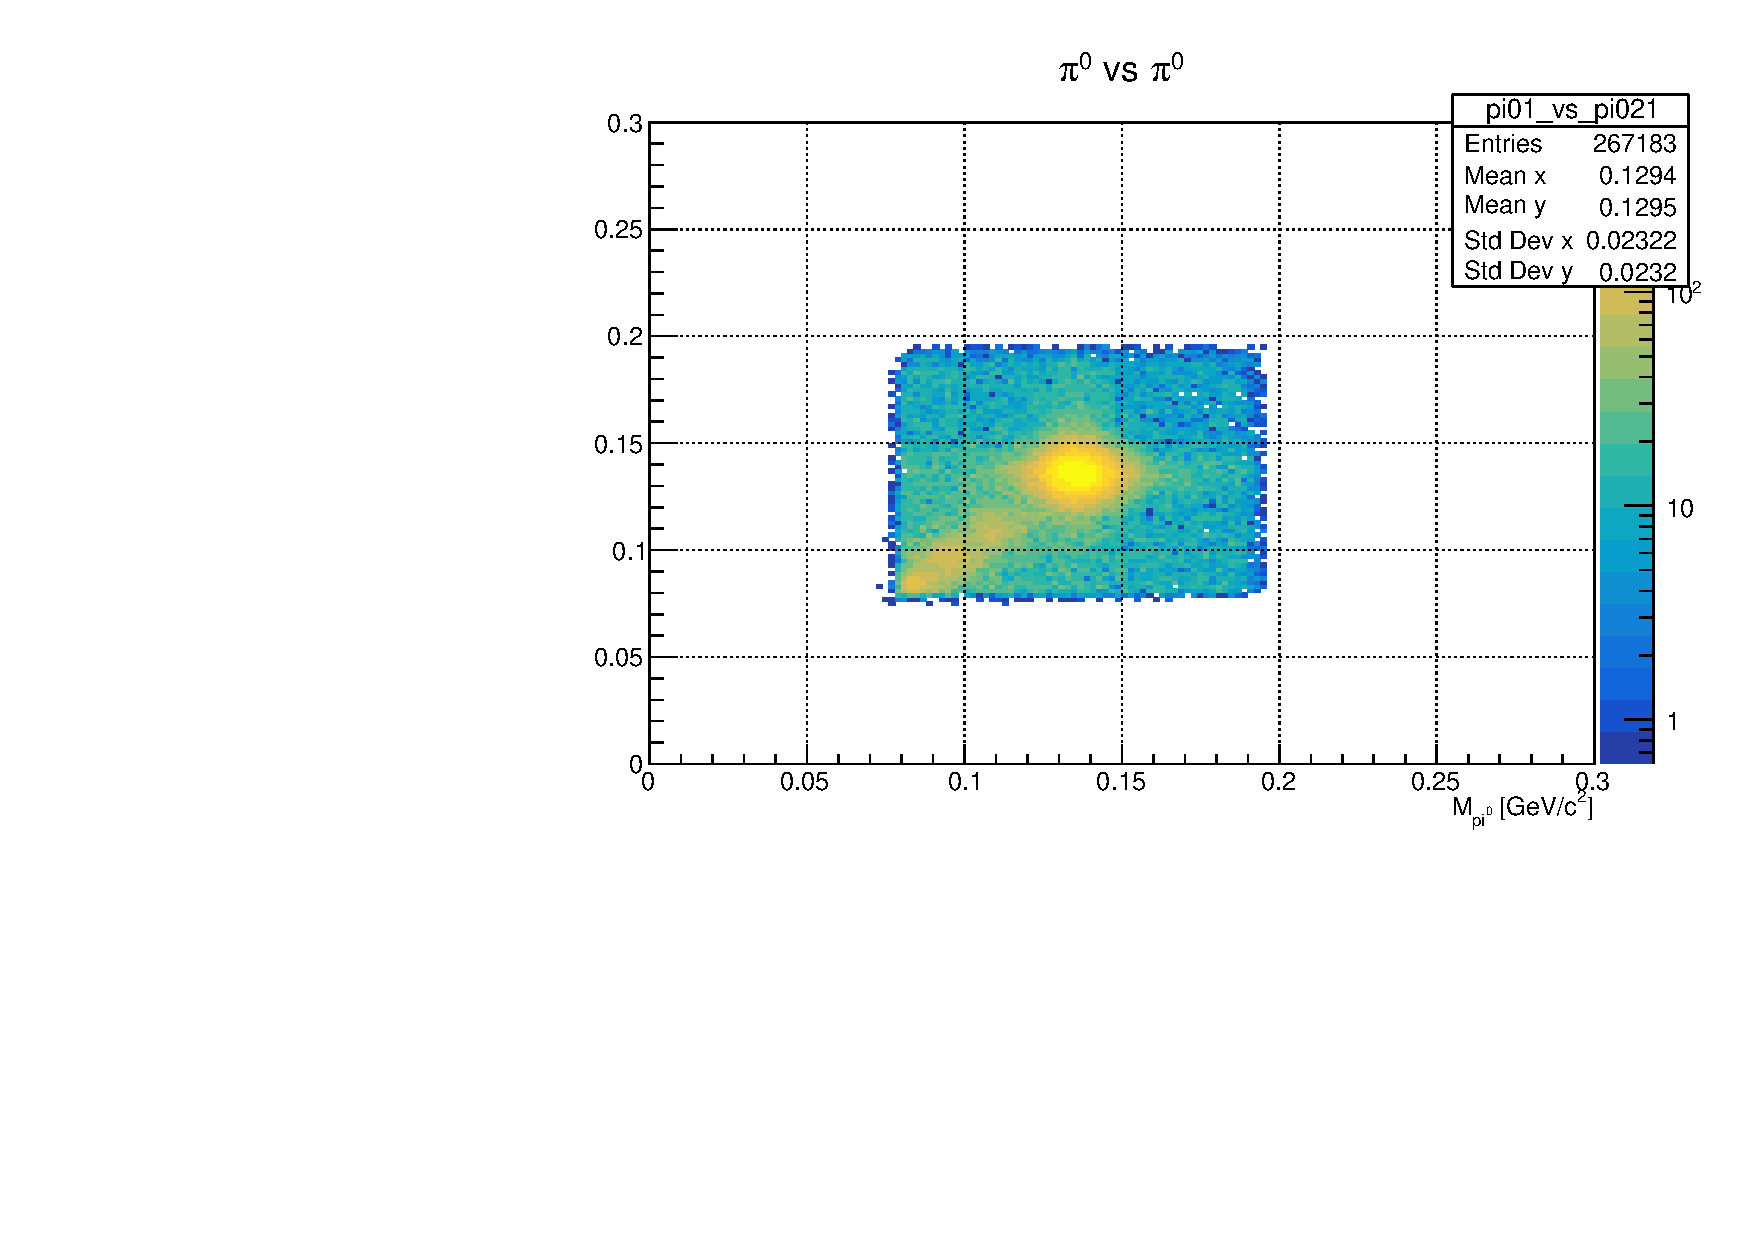
\includegraphics[width=4.75in]{figures/pi0VSpi0.pdf} \\
\centering
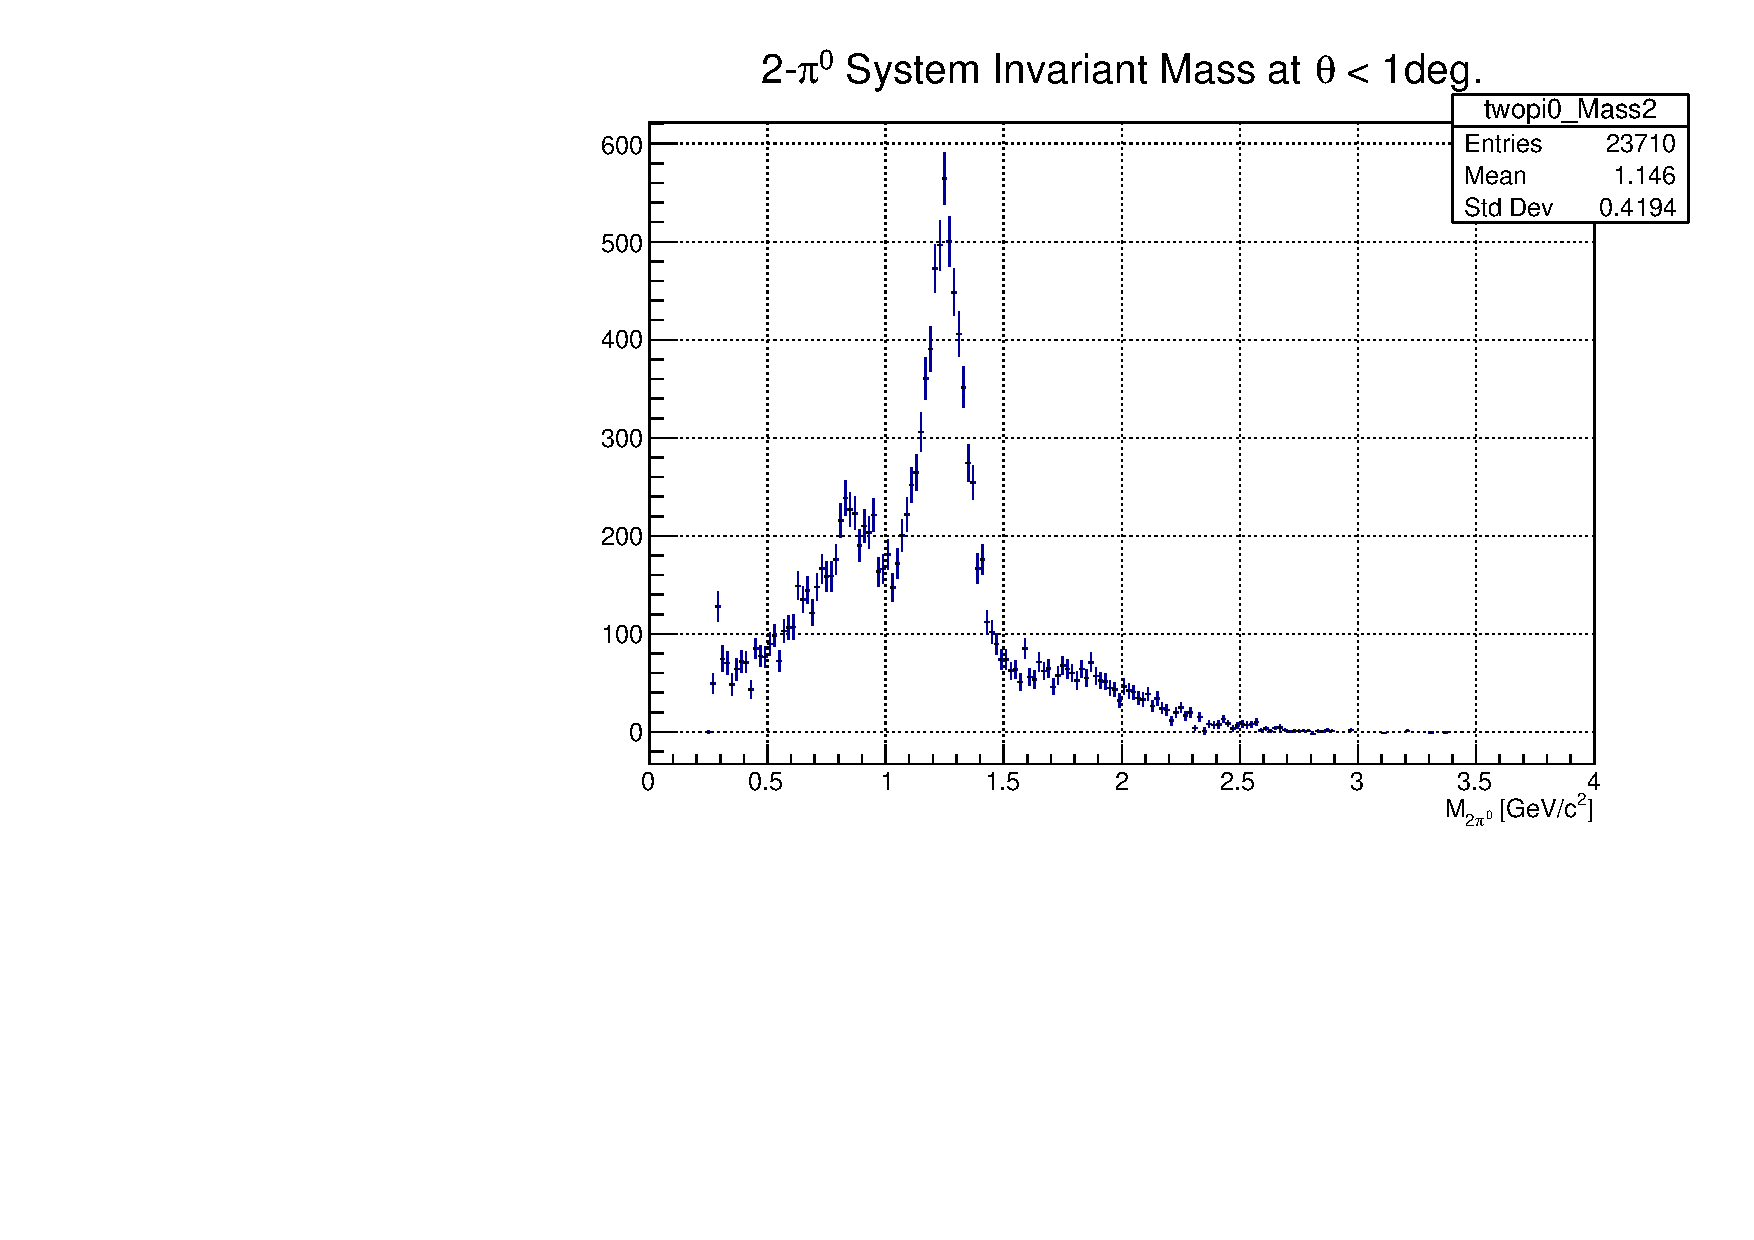
\includegraphics[width=4.75in]{figures/TwoPiInvMass.pdf}
\caption{Experimental distributions from the 2017 GlueX data set
  analyzed as $\gamma p\rightarrow \gamma \gamma \gamma \gamma\, (p)$
  with a missing proton. Top: Two photon invariant mass of one pair vs
  the two photon invariant mass of the second pair. Bottom: 2$\pi$
  mass distribution selecting events with the reconstructed photon
  pair masses close to the $\pi^0$ mass as shown above. The plot also
  requires that the angle of the two-pion system be less than 1
  degree.
\label{fig:TwoPiInvMass}}
\end{figure}

The invariant mass distribution in two dimensions, for a given photon pair versus that for
the other pair in these four-photon events shows a
strong $\pi^0$ peak, as shown in the top of
Fig.~\ref{fig:TwoPiInvMass}. There are background events that fall
under the two $\pi^0$ peaks, which require further study,
nevertheless, using the selection of photon pairs that reconstruct to
the $\pi^0$, we can plot the 2$\pi^0$ mass spectrum (bottom of
Fig.~\ref{fig:TwoPiInvMass}). The mass spectrum has recognizable
features, in particular the prominent $f_2(1270)$ that decays to
$\pi^0\pi^0$ 85\% of the time. The structure at $M_{\pi\pi}\sim$0.8~GeV
appears too low for the $f_0(980)$ and is present in a location
where the Crystal Ball data \cite{Marsiske:1990hx} shows a low
yield. The yield for $M_{\pi\pi}<$0.5 GeV is consistent within a
factor of two of the relative yield compared to the $f_2(1270)$ peak in
the Crystal Ball data. This analysis demonstrates that these neutral
events can be analyzed in our detector under circumstances significantly more
challenging than we anticipate for the Primakoff
experiment. In particular, for the Primakoff experiment, we will have
a solid nuclear target with little extent in $z$ that will allow valid geometrical constraints
and thus improving the resolution on missing momentum in the reaction. This will
make the kinematic fitting more effective.

It is evident from the top plot in Fig.~\ref{fig:TwoPiInvMass} that a cut
on the invariant mass of one reconstructed $\pi^{0}$ will reduce the
background on the other $\pi^{0}$ significantly. This is shown in
Fig.~\ref{fig:pi0yield} where a cut on the invariant of one $\pi^{0}$
significantly reduces the background in the other while keeping the
main signal mostly undisturbed.
\begin{figure}[htp]
\centering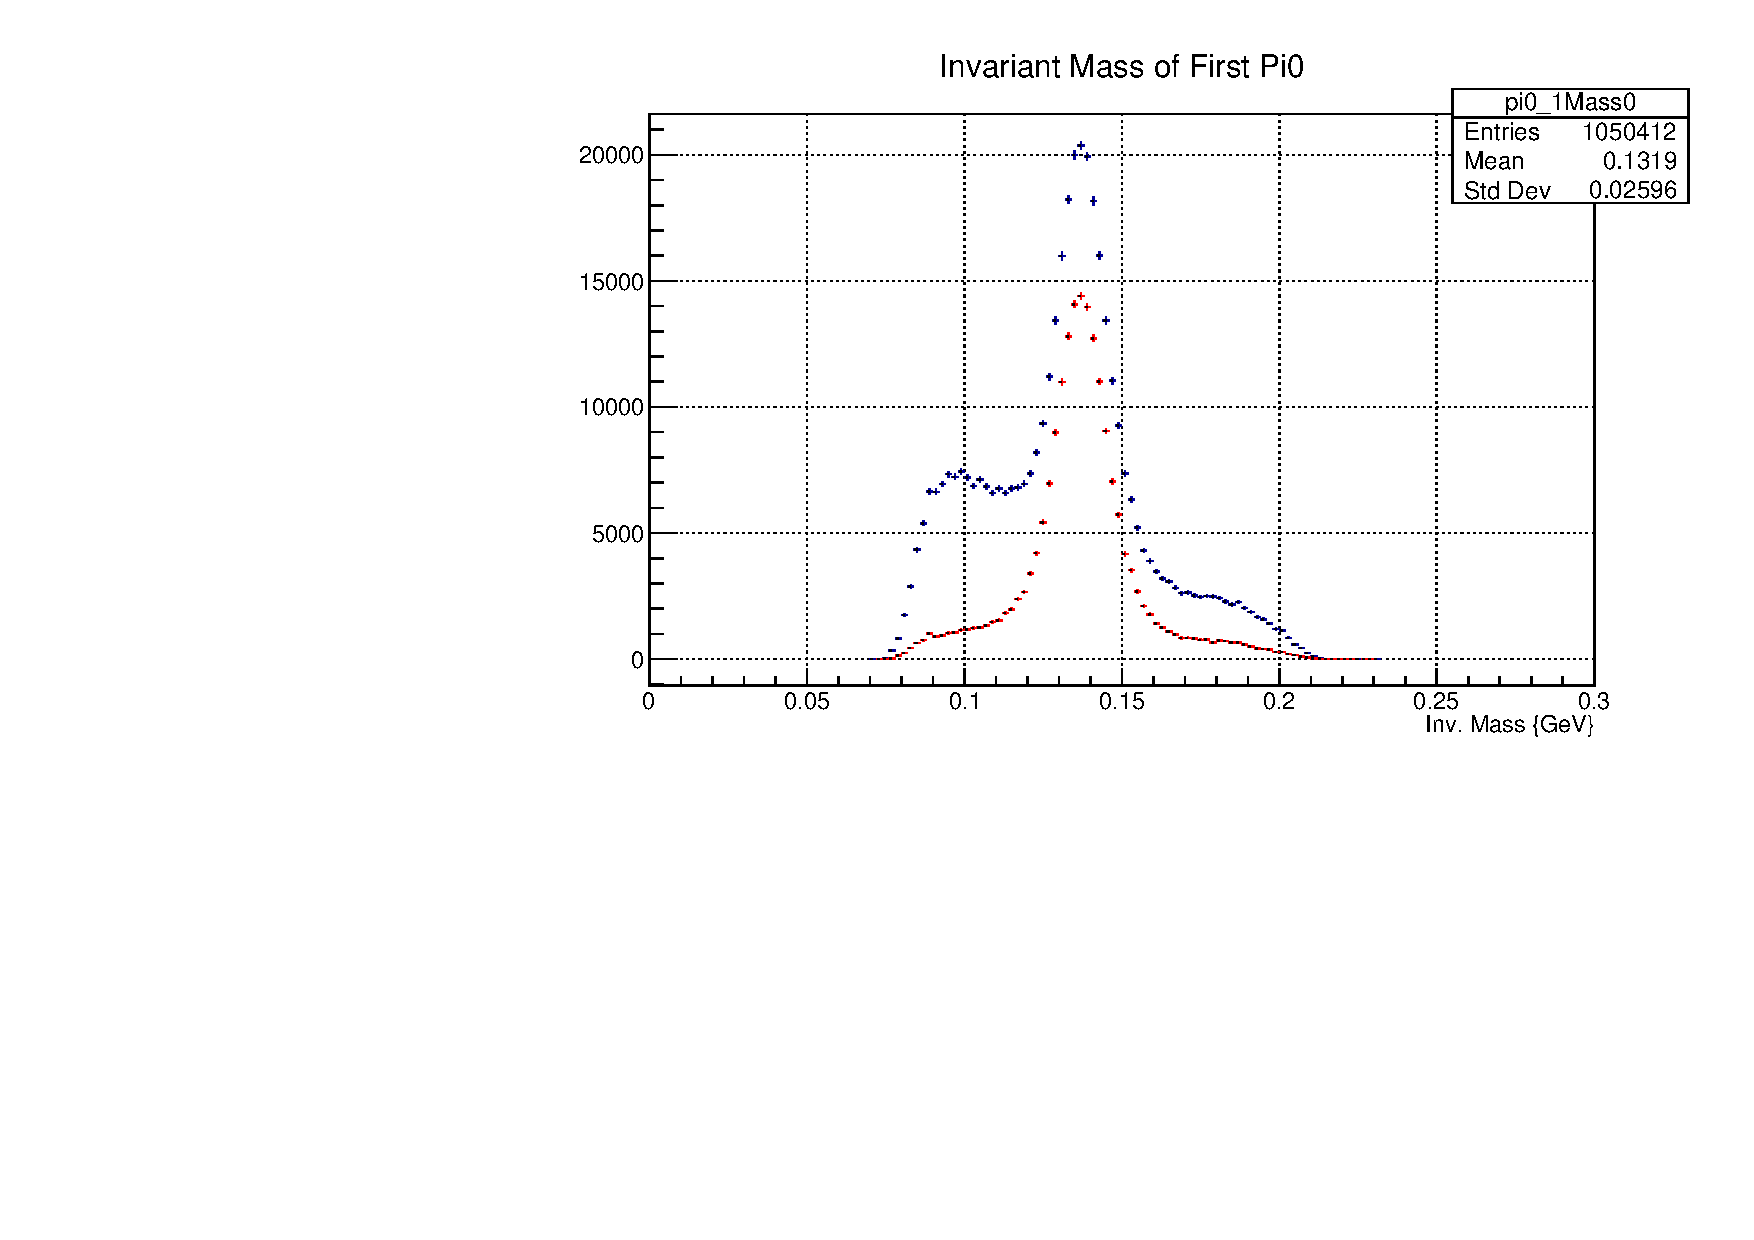
\includegraphics[width=4.75in]{figures/pi0_inv_mass_withpi02cut.pdf}
\caption{Invariant mass of the two-photon system with (red) and
  without (blue) a cut on the invariant mass of the second pair of
  photons.
\label{fig:pi0yield}}
\end{figure}

These photons are detected by the lead-glass calorimeter whose energy resolution is the
main contribution to the resolution of the reconstructed $\pi^{0}$
mass. A lead-tungstate calorimeter with a substantially better energy
resolution would yield a significant improvement in the signal-to-noise
ratio as the width of the reconstructed $\pi^{0}$ would be
smaller by about a factor of two.

\subsection{Helium and beryllium targets}

The PrimEx-Eta experiment collected valuable data on light nuclear
targets ($^4$He and $^9$Be) in 2019. Analysis of two-neutral-pion-system
photoproduction on these nuclei gives a good estimate of the
main background sources, signal-to-background levels, and the Hall-D
detector resolution for the main kinematic variables. The total PrimEx-Eta luminosity
corresponds to approximately one day on
a 5\% radiation length beryllium target and 18 days on a
4\% radiation length helium target at 200~nA electron beam
current and a $10^{-4}$ radiation length amorphous tagger
radiator. The beryllium target has a thickness of only 1.5~cm
(compared to the 30~cm liquid helium and hydrogen targets), which allows
constraining interaction point (important for reconstruction of neutral pions
without any additional vertex information from the
tracking system).  First we identified the two neutral pion
process using the ratio of energy of the two pions to the
initial beam energy with the expected recoil energy
subtracted. Fig.$\,$\ref{fig:pi0elastbe} shows this distribution for
pions detected in FCAL and time accidentals and out-of-target beam
interaction subtracted.
\begin{figure}[!h]
\centering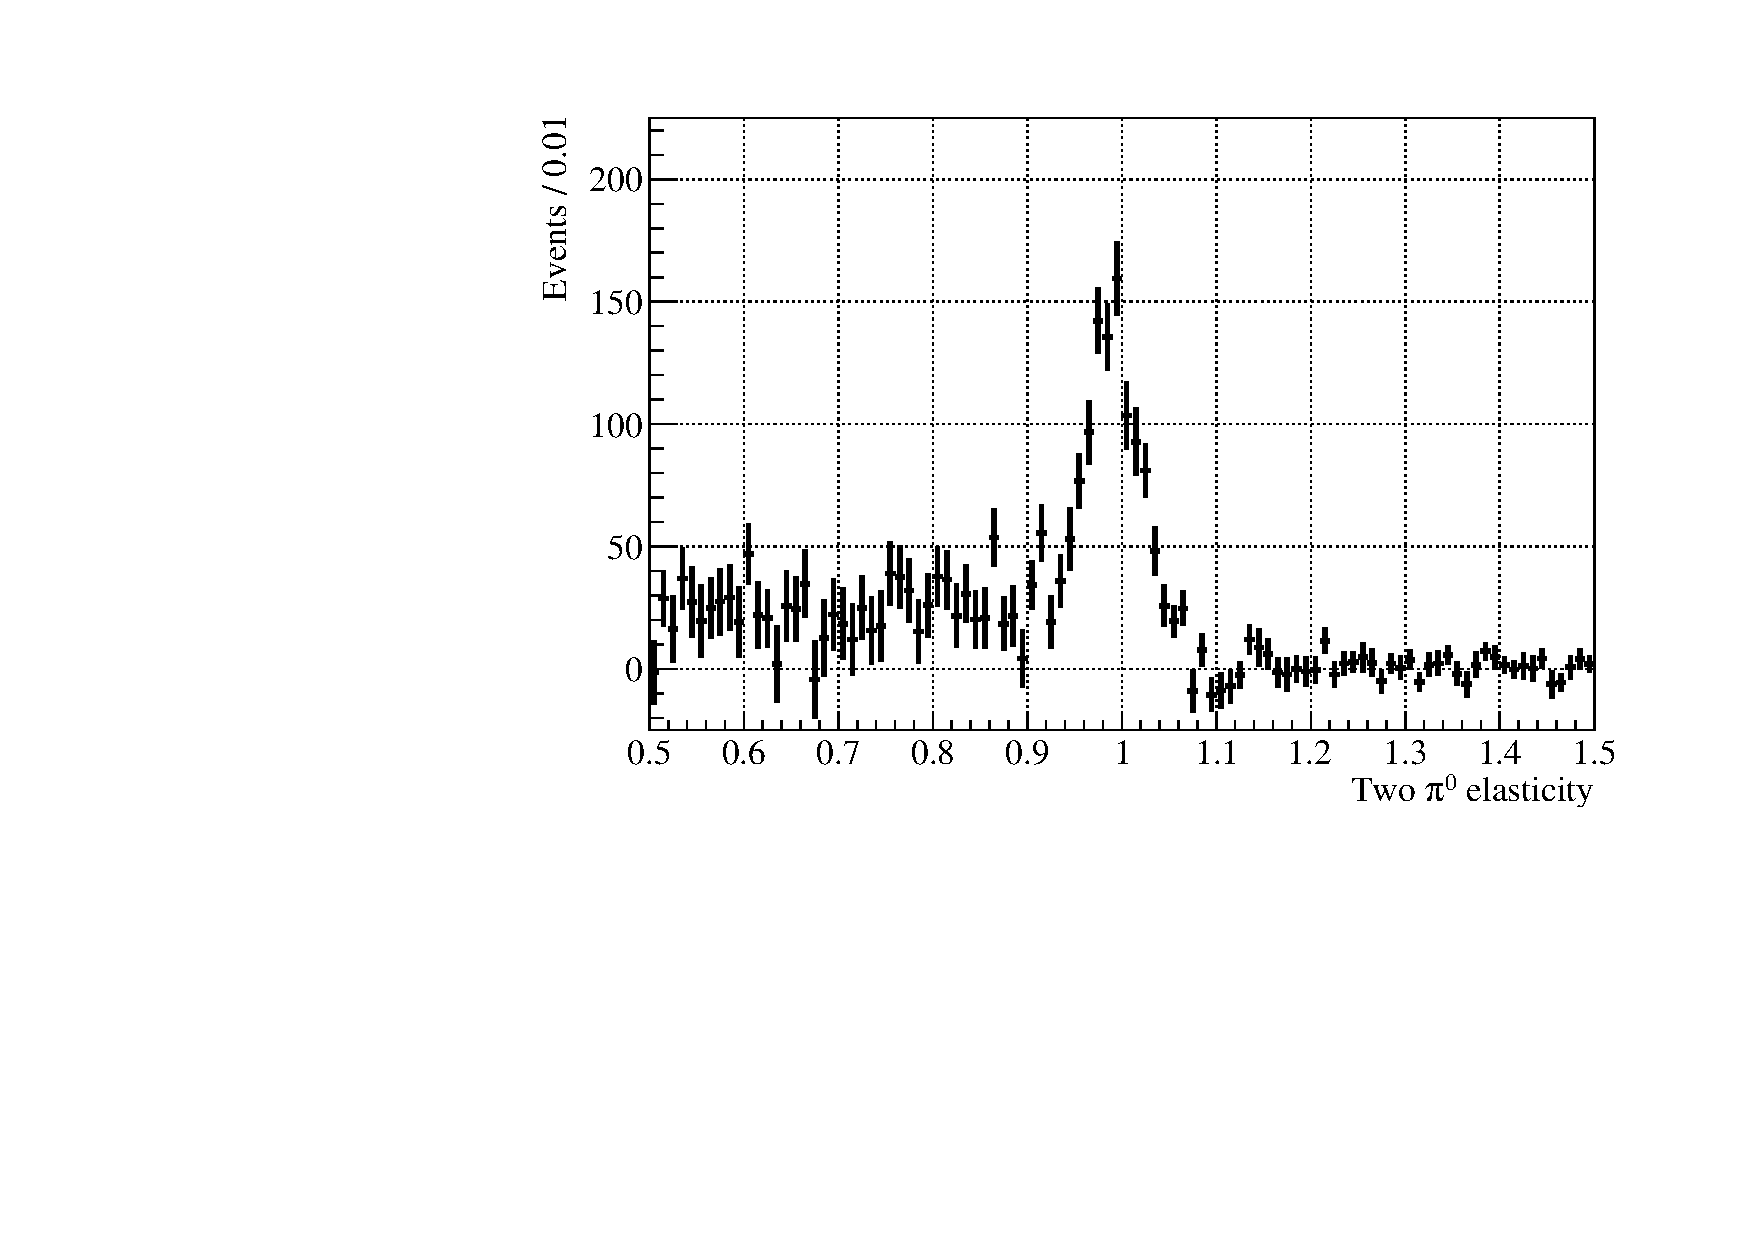
\includegraphics[width=4.75in]{figures/be_elast1.pdf}
\caption{Two neutral pion elasticity (ratio of two-pion energy to that expected for exclusive production) for the beryllium target.
\label{fig:pi0elastbe}}
\end{figure}
We first required exactly four showers to be detected in FCAL and no
extra showers in BCAL and COMCAL, a minimum shower energy of
0.5~GeV, and no neutral signals in the time-of-flight detector. The number of the signal
events here is about 900, the width of the observed signal with a
kinematic fit to the pion mass is about 3\%, and the signal-to-background
ratio value is promising. Fig.~\ref{fig:2dbe} shows the two
dimensional distribution of these events: elasticity vs.\ invariant
mass. One can see the horizontal line of the exclusive production
events and the vertical line of $K_S\to\pi^0\pi^0$ decays, which are
separated from each other. Presence of $K_S\to\pi^0\pi^0$ decays
in the data is really beneficial for the Primakoff analysis since it
allows tuning the detector resolution in Monte Carlo and making an
assessment of the level of agreement with the data, which
is essential for the successful cross section fitting procedure and
systematic uncertainty control.
\begin{figure}[!h]
\centering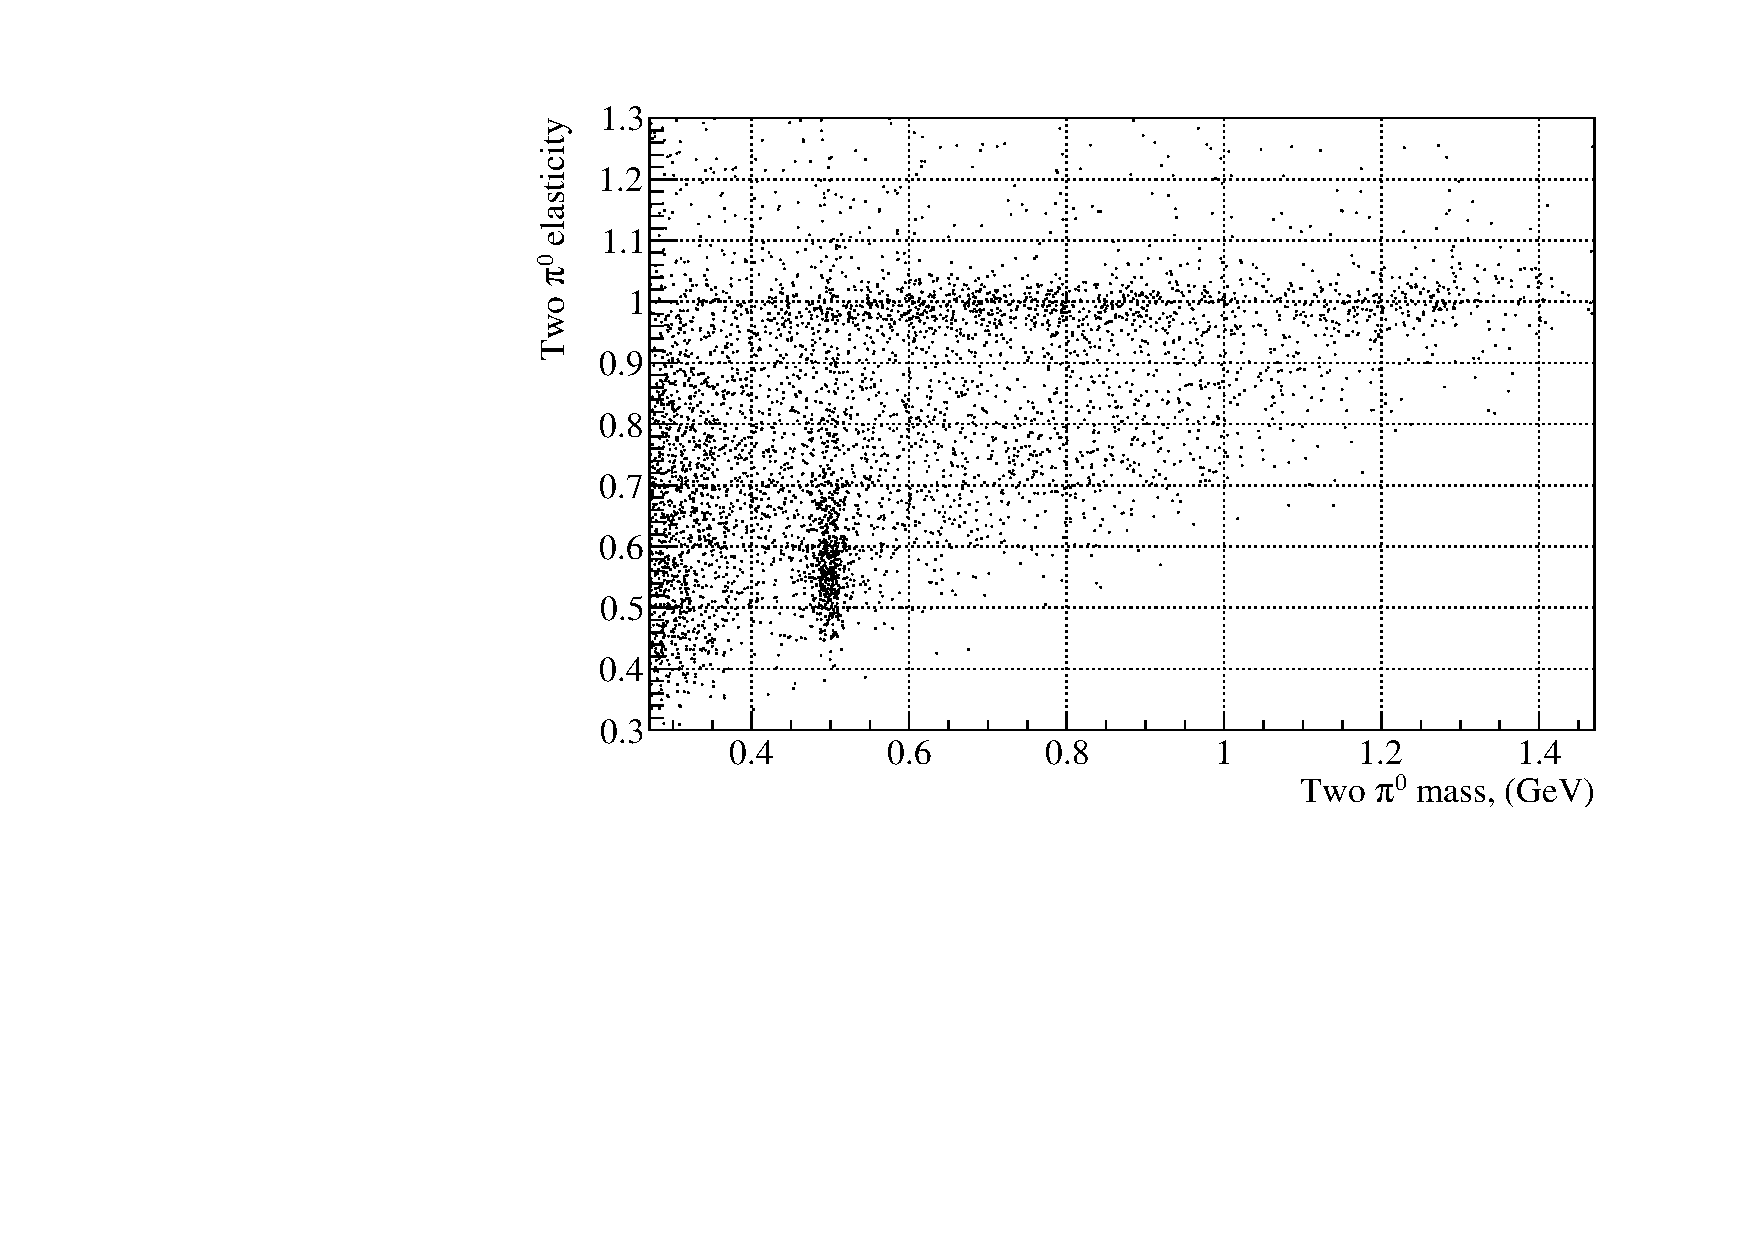
\includegraphics[width=4.75in]{figures/2d_be.pdf}
\caption{Two neutral pion elasticity (ratio of two-pion energy to that expected
  for exclusive production) vs.\ invariant mass of two pions
  for the beryllium target.
\label{fig:2dbe}}
\end{figure}

Including BCAL showers in the neutral pion reconstruction increases
the acceptance (especially for the large invariant mass region) and the number
of observed events goes up by an order of magnitude. For the beryllium target
this increases the number of exclusive events to $\sim 10$~k and for
the helium target to $\sim 200$~k events. Fig.~\ref{fig:bemass}
shows the two $\pi^0$ invariant mass distribution. These data have the BCAL included,
the two-pion energy is required to be within
10\% of that expected for exclusive events, and the production angle
of the two-pion system was required to be below one degree. The $f_2$ meson
peak is clearly seen. Fig.~\ref{fig:beheelast} shows the elasticity
distribution for both helium and beryllium targets with BCAL
reconstruction included (time accidentals and empty target
background subtracted).
\begin{figure}[!h]
\centering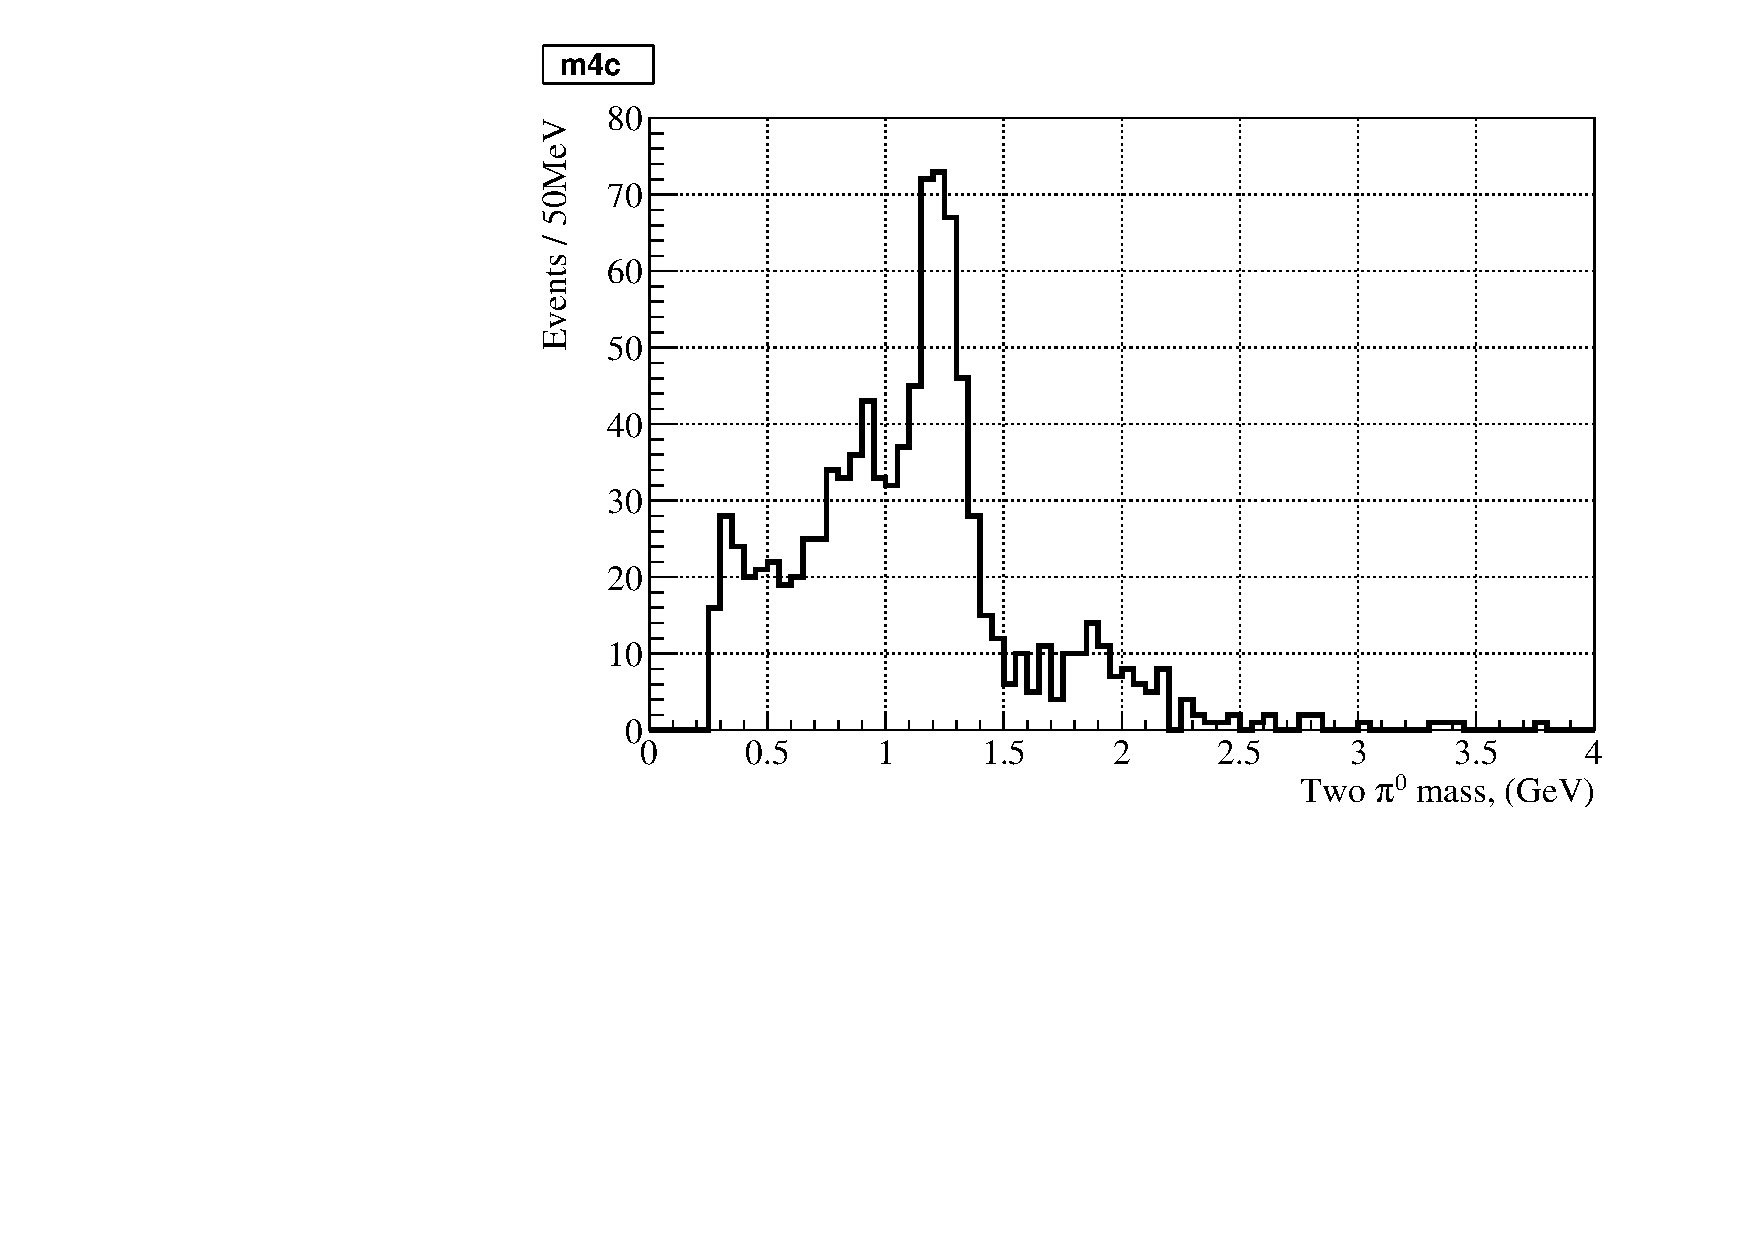
\includegraphics[width=4.75in]{figures/be_mass.pdf}
\caption{Two neutral pion invariant mass for the exclusive events
  (i.e., within 10\% of the expected energy). Data from the beryllium target. The production angle
  was required to be below one degree.
\label{fig:bemass}}
\end{figure}
\begin{figure}[!h]
\centering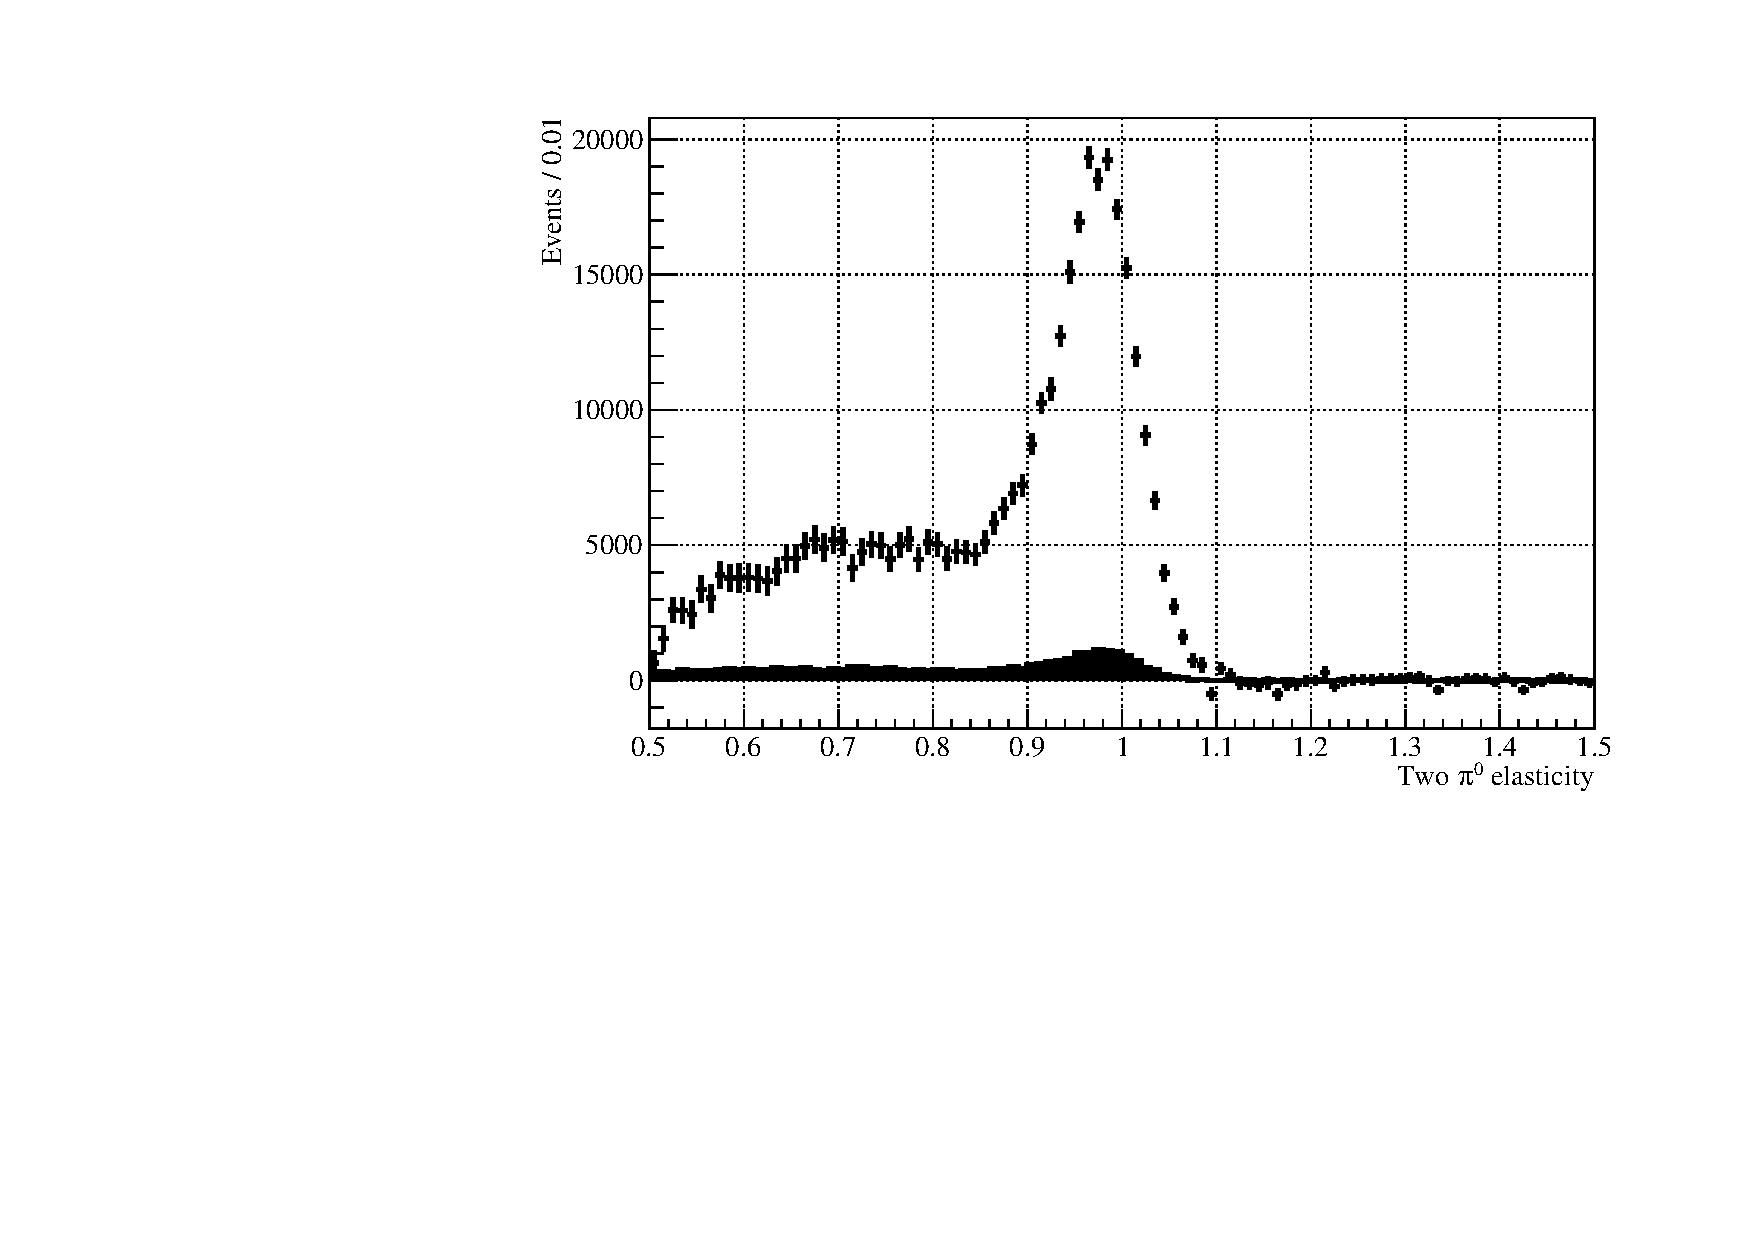
\includegraphics[width=4.5in]{figures/hebe_elast.pdf}
\caption{The two-pion elasticity distribution with BCAL included in the
  analysis. Empty target data and time accidentals are subtracted. Open
  histogram: helium target, $\sim 200$~k events in the elastic
  peak. Solid histogram: beryllium target, $\sim 10$~k events in
  the peak.
\label{fig:beheelast}}
\end{figure}

We wish to highlight the good detector
resolution for two $\pi^0$ production kinematics variables, the
presence of the calibration process ($K_S$) in the data and the
controllable level of backgrounds observed for light nuclear target
exposure.
